%%%%%%%%%%%%%%%%%%%%%%%%%%%%%%%%%%%%%%%%%%%%%%%%%%%%%%%%%%%%%%%%%%%%%%
% Skupina16/main.tex
% Slike: Skupina16/img/ (ustvari jih skripta slike.py v korenu repozitorija iz results/).
%%%%%%%%%%%%%%%%%%%%%%%%%%%%%%%%%%%%%%%%%%%%%%%%%%%%%%%%%%%%%%%%%%%%%%

\graphicspath{{Skupina16/img/}}

\title{Kje Groverjev algoritem preneha delovati na IBM Heron? Napoved praga z digitalnim dvojčkom iz kalibracijskih podatkov}
\titlerunning{Prag Groverjevega algoritma na IBM Heron}
\author{Gašper Jug}
\maketitle

\abstract{Zanimalo nas je, pri kolikšnem številu kubitov $n$ Groverjev algoritem na procesorju IBM Heron (\texttt{ibm\_marrakesh}) ne da več uporabnega rezultata in ali ta prag napove šumni simulator (digitalni dvojček), zgrajen iz kalibracijskih podatkov procesorja. Vezja za $n = 2 \ldots 6$ smo v Qiskitu prevedli enkrat in jih pognali na idealnem simulatorju, na treh dvojčkih in v treh nalogah na procesorju. Pri $n = 5$ (okoli 520 vrat CZ) je verjetnost uspeha na procesorju v petih od šestih vezij jasno nad dvakratnikom naključnega ugibanja (\num{0,092}--\num{0,106} proti \num{0,0625}), v enem (\num{0,064}) pa na meji; pri $n = 6$ (okoli \num{1800}--\num{2100} vrat CZ) je v vseh zagonih na ravni naključnega ugibanja (\num{0,013}--\num{0,017}). Vsi dvojčki prag napovejo pravilno, verjetnost uspeha pa precenijo: pri $n = 5$ za \num{1,2}- do \num{1,3}-krat, če upoštevajo dekoherenco kubitov med čakanjem, in za \num{2,1}-krat, če je ne. Ob štetju klasičnih poizvedb je Groverjev algoritem na procesorju hitrejši od klasičnega iskanja le do $n = 3$. Dvojček iz kalibracije je torej uporaben za napoved praga, ne pa za natančno napoved verjetnosti uspeha.}


\section{Uvod}
\label{g16:sec:uvod}

Groverjev algoritem~\cite{grover1996} poišče označen element v neurejeni množici $N = 2^n$ elementov. Uporablja orakelj, torej funkcijo, ki za dani element pove, ali je označen, in ga pokliče le $O(\sqrt{N})$-krat, klasično iskanje pa potrebuje v povprečju $N/2$ poizvedb. Po $k$ ponovitvah oraklja in difuzije je verjetnost, da izmerimo označeno stanje,
\begin{equation}
P_\mathrm{ideal}(k) = \sin^2\!\big((2k+1)\,\theta\big), \qquad \theta = \arcsin\frac{1}{\sqrt{N}},
\label{g16:eq:pideal}
\end{equation}
ki je pri $k = \lfloor \frac{\pi}{4}\sqrt{N} \rfloor$ blizu 1~\cite{nielsen2010}. Na idealnem simulatorju algoritem torej ne odpove, omejitev je le pomnilnik za $2^n$ amplitud.

Današnji kvantni procesorji so šumni~\cite{preskill2018}. Večkrat kontrolirana vrata v oraklju in difuziji se razstavijo v veliko dvokubitnih vrat, kubiti niso povezani vsak z vsakim, zato prevajalnik doda vrata SWAP, napake vrat, odčitavanja in dekoherence pa se z dolžino vezja seštevajo. Idealni vrh pri označenem stanju se zato razmaže proti enakomerni porazdelitvi z verjetnostjo $1/2^n$. Pri nekem $n$ algoritem ne da več uporabnega rezultata.

Ker je čas na procesorjih omejen, poskuse pogosto najprej izvedemo na šumnem simulatorju, ki iz kalibracijskih podatkov procesorja (časi $T_1$, $T_2$, napake vrat in odčitavanja) zgradi model šuma. Takemu simulatorju pravimo digitalni dvojček. V tem delu dvojčke preverjamo na procesorju IBM Heron~\cite{g16:ibm_processors} na konkretnem algoritmu z znanim idealnim rezultatom in klasično primerjavo ter preverimo, kako na napoved vplivata vir kalibracijskih podatkov in dekoherenca kubitov med čakanjem.

\begin{svgraybox}
\textbf{Raziskovalno vprašanje.} Pri kolikšnem številu kubitov $n$ Groverjev algoritem na procesorju IBM Heron (\texttt{ibm\_marrakesh}) preneha dajati uporaben rezultat in ali ta prag napove digitalni dvojček, zgrajen iz kalibracijskih podatkov procesorja?

\textbf{Pričakovani rezultat.} Prag je pri $n^* = 5 \pm 1$: verjetnost uspeha pade pod dvakratnik naključnega ugibanja med $n = 5$ in $n = 6$. Dvojček prag napove znotraj enega kubita, verjetnost uspeha pa precenjuje, ker ne zajame vseh napak.
\end{svgraybox}

V razdelku~\ref{g16:sec:metode} opišemo vezja, dvojčke in metrike, v razdelku~\ref{g16:sec:rezultati} rezultate treh nalog na procesorju, v razdelku~\ref{g16:sec:razprava} pa odgovor na vprašanje, omejitve in poskuse, ki niso uspeli.


\section{Metode}
\label{g16:sec:metode}

\subsection{Orodja in nastavitve}
\label{g16:sec:orodja}

Vezja smo zapisali v Qiskitu~\cite{qiskit2024}, simulirali s Qiskit Aer in izvedli prek IBM Quantum Open Plan. Nastavitve, ki vplivajo na rezultat, so zbrane v tabeli~\ref{g16:tab:orodja}. Koda, kalibracijski podatki in vsi rezultati so v repozitoriju skupaj z navodili za ponovitev.

\begin{table}[htbp]
\caption{Orodja in nastavitve poskusov.}
\label{g16:tab:orodja}
\centering
\begin{tabular}{ll}
\toprule
Nastavitev & Vrednost \\
\midrule
Python, Qiskit & 3.12.3, 2.6.2 \\
qiskit-aer, qiskit-ibm-runtime & 0.18.2, 0.52.1 \\
procesor & \texttt{ibm\_marrakesh} (IBM Heron, 156 kubitov) \\
osnovna vrata & CZ, $\sqrt{X}$, $X$, $R_Z$ \\
prevajanje & \texttt{transpile}, stopnji 1 in 3, \texttt{seed\_transpiler=1} \\
ponovitve (QPU in simulacije) & \num{10000} na vezje \\
naloge na QPU & 3, vsaka z 10 vezji ($n = 2 \ldots 6$, stopnji 1 in 3) \\
izvajanje & \texttt{SamplerV2}, privzete nastavitve \\
\bottomrule
\end{tabular}
\end{table}

\subsection{Zasnova poskusov}
\label{g16:sec:poskusi}

\textbf{Vezja.} Za vsak $n = 2 \ldots 6$ smo naključno izbrali označeno stanje (seme 7) in zgradili Groverjevo vezje s $k = \lfloor \frac{\pi}{4}\sqrt{2^n} \rfloor$ ponovitvami. Orakelj z vrati $X$ preslika označeno stanje v $\ket{1\ldots1}$, nanj deluje z $(n-1)$-krat kontroliranimi vrati $Z$ in preslikavo razveljavi, difuzija pa je $H^{\otimes n} X^{\otimes n} (C^{n-1}Z) X^{\otimes n} H^{\otimes n}$. Pomožnih kubitov ne uporabljamo. Slika~\ref{g16:fig:vezje} prikazuje eno ponovitev za $n = 3$, tabela~\ref{g16:tab:vrata} pa delovanje vseh vrat, ki se pojavijo v vezjih in pri njihovem prevajanju.

\begin{table}[htbp]
\caption{Kvantna vrata v vezjih in pri prevajanju~\cite{nielsen2010}. Fazo, ki je skupna vsem stanjem (globalna faza), izpuščamo, ker ne vpliva na meritev.}
\label{g16:tab:vrata}
\centering
\small
\begin{tabularx}{\textwidth}{lX}
\toprule
Vrata & Delovanje \\
\midrule
$H$ & $\ket{0} \to (\ket{0}+\ket{1})/\sqrt{2}$, $\ket{1} \to (\ket{0}-\ket{1})/\sqrt{2}$; iz $\ket{0\ldots0}$ ustvarijo enakomerno superpozicijo vseh stanj \\
$X$ & zamenja $\ket{0}$ in $\ket{1}$ (kvantni NE) \\
$\sqrt{X}$ & polovica vrat $X$ (rotacija za $\pi/2$ okoli osi $x$), $\sqrt{X}\sqrt{X} = X$ \\
$R_Z(\varphi)$ & stanju $\ket{1}$ doda fazo $e^{i\varphi}$, $\ket{0}$ pusti; vrata $T$ in $T^\dagger$ sta $R_Z(\pm\pi/4)$ \\
CNOT & zamenja $\ket{0}$ in $\ket{1}$ na ciljnem kubitu, če je kontrolni kubit v $\ket{1}$ \\
CZ & obrne predznak stanja $\ket{11}$; vloga obeh kubitov je enaka \\
$C^{n-1}Z$ & obrne predznak stanja $\ket{1\ldots1}$ na $n$ kubitih ($CCZ$ za $n = 3$) \\
SWAP & zamenja stanji dveh kubitov; razstavi se v 3 vrata CNOT oziroma CZ \\
\bottomrule
\end{tabularx}
\end{table}

\begin{figure}[htbp]
\centering
\begin{quantikz}[column sep=0.25cm, row sep=0.2cm]
\lstick{$q_0$} & \gate{H} & \gate{X} & \ctrl{1}  & \gate{X} & \gate{H} & \gate{X} & \ctrl{1}  & \gate{X} & \gate{H} & \qw \\
\lstick{$q_1$} & \gate{H} & \gate{X} & \ctrl{1}  & \gate{X} & \gate{H} & \gate{X} & \ctrl{1}  & \gate{X} & \gate{H} & \qw \\
\lstick{$q_2$} & \gate{H} & \qw      & \control{} & \qw     & \gate{H} & \gate{X} & \control{} & \gate{X} & \gate{H} & \qw
\end{quantikz}
\caption{Groverjevo vezje za $n = 3$ in označeno stanje $\ket{100}$ (kubit $q_2$ je najvišji bit): začetni vrata $H$, nato orakelj (vrata $X$ na kubitih, kjer ima označeno stanje ničlo, in vrata $CCZ$) ter difuzija. Pri $n = 3$ se orakelj in difuzija ponovita $k = 2$-krat.}
\label{g16:fig:vezje}
\end{figure}

\textbf{Prevajanje.} Transpiler vezje prevede v več korakih: izbere fizične kubite (postavitev), doda vrata SWAP, kjer vrata delujejo med nesosednjimi kubiti (usmerjanje), razstavi vsa vrata v osnovna vrata procesorja in vezje optimizira. Stopnja optimizacije (0--3) določa, koliko truda vloži v zadnji korak. Stopnja 1 le združi zaporedna enokubitna vrata v ena in odstrani pare vrat, ki se izničijo. Stopnja 3 poleg tega zaporedja vrat na istem paru kubitov nadomesti z najkrajšo enakovredno razstavitvijo, izkoristi zamenljivost vrat in preizkusi več usmerjanj, od katerih obdrži najboljše. Pri stopnji 3 ima vezje do 18~\% manj vrat CZ (tabela~\ref{g16:tab:vezja}). Vsako vezje smo prevedli za procesor \emph{enkrat}; isto prevedeno vezje gre na procesor in v vse simulatorje, zato prevajanje ne vpliva na primerjavo. Pri stopnji 1 je transpiler izbral fizične kubite, pri stopnji 3 pa smo mu predpisali isto postavitev (\texttt{initial\_layout}), da se stopnji razlikujeta le v optimizaciji vrat. Kubiti procesorja so povezani v mrežo težkega šestkotnika, v kateri ima vsak kubit največ tri sosede~\cite{g16:ibm_processors}, vrata CZ pa delujejo le med sosedi. Vrata $R_Z$ procesor izvede programsko, s trajanjem in napako 0~\cite{g16:mckay2017,g16:ibm_qpuinfo}, zato šum prinašajo le vrata CZ, $\sqrt{X}$ in $X$ ter čakanje. Tabela~\ref{g16:tab:vezja} prikazuje lastnosti vezij pred prevajanjem in po njem. Število dvokubitnih vrat raste hitreje od $\sqrt{N}$, ker se večkrat kontrolirana vrata brez pomožnih kubitov razstavijo v vse več vrat: vrata $CCZ$ potrebujejo 6 vrat CNOT (slika~\ref{g16:fig:ccz}), $C^3Z$ 14, $C^4Z$ 36 in $C^5Z$ 82.

\begin{figure}[htbp]
\centering
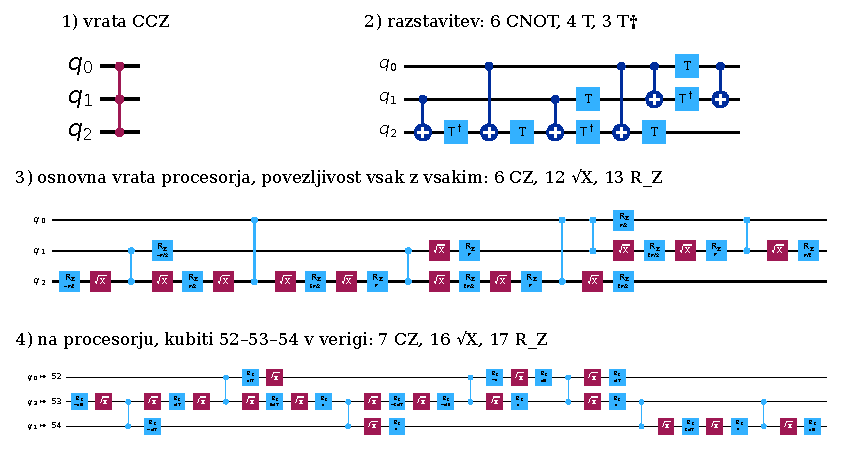
\includegraphics[width=\textwidth]{kaskada_ccz}
\caption{Koraki prevajanja vrat $CCZ$: (1) logična vrata; (2) razstavitev v 6 vrat CNOT in 7 vrat $T$, $T^\dagger$~\cite{nielsen2010}; (3) osnovna vrata procesorja pri povezljivosti vsak z vsakim: 6 vrat CZ, 12 $\sqrt{X}$ in 13 $R_Z$; (4) na procesorju, kjer so kubiti 52--53--54 povezani v verigo: 7 vrat CZ, 16 $\sqrt{X}$ in 17 $R_Z$. Razstavitve so ustvarjene s Qiskitom in preverjene kot enakovredne vratom $CCZ$.}
\label{g16:fig:ccz}
\end{figure} Omejena povezljivost doda še SWAP-e: po prevajanju ima vezje \num{1,5}- do \num{2,3}-krat več dvokubitnih vrat kot pri povezljivosti vsak z vsakim.

\begin{table}[htbp]
\caption{Lastnosti vezij. Globina je število zaporednih plasti vrat, torej najdaljša pot vrat, ki se morajo izvesti eno za drugim. \emph{Pred prevajanjem}: logično vezje, globina po razstavljanju večkrat kontroliranih vrat in število vrat CX pri povezljivosti vsak z vsakim. \emph{Po prevajanju}: vezje za \texttt{ibm\_marrakesh} pri stopnji 1 / 3.}
\label{g16:tab:vezja}
\centering
\begin{tabular}{rrrrrrr}
\toprule
 & & \multicolumn{2}{c}{pred prevajanjem} & \multicolumn{2}{c}{po prevajanju} & \\
\cmidrule(lr){3-4}\cmidrule(lr){5-6}
$n$ & $k$ & globina & CX & globina & CZ & $P_\mathrm{ideal}$ \\
\midrule
2 & 1 & 12 & 2 & 12 / 9 & 2 / 2 & \num{1,000} \\
3 & 2 & 58 & 24 & 169 / 135 & 45 / 37 & \num{0,945} \\
4 & 3 & 178 & 84 & 662 / 495 & 189 / 163 & \num{0,961} \\
5 & 4 & 690 & 288 & \num{1841} / \num{1441} & 549 / 517 & \num{0,999} \\
6 & 6 & \num{1539} & 984 & \num{5305} / \num{4334} & \num{2073} / \num{1773} & \num{0,997} \\
\bottomrule
\end{tabular}
\end{table}

\textbf{Digitalni dvojčki.} Vsi dvojčki uporabljajo isto standardno konstrukcijo Qiskit Aer, \texttt{NoiseModel.from\_backend}~\cite{g16:aer_noisemodel}, ki vsakemu kubitu in paru kubitov pripiše termično relaksacijo ($T_1$, $T_2$, trajanje vrat), depolarizacijski šum in napako odčitavanja. Depolarizacijski del izbere tako, da je skupna povprečna napaka vrat enaka sporočeni napaki iz kalibracije~\cite{g16:magesan2011}, zato dekoherenca med vrati ni šteta dvakrat. Vezja pred simulacijo razporedimo (ALAP), tako da je čas, ko kubit čaka na druge, zapisan kot ukaz \texttt{delay}, na katerem model doda termično relaksacijo. Dvojčki se razlikujejo le po izvoru kalibracije (tabela~\ref{g16:tab:dvojcki}). Kalibracijski CSV smo pretvorili v objekt \texttt{Backend} tako, da smo v \texttt{FakeMarrakesh} (od koder vzamemo le povezljivost in nabor vrat) vpisali vrednosti iz datoteke (izpis~\ref{g16:lst:dvojcek}).

\begin{table}[htbp]
\caption{Digitalni dvojčki. Vsi uporabljajo \texttt{NoiseModel.from\_backend}.}
\label{g16:tab:dvojcki}
\centering
\begin{tabular}{lll}
\toprule
Dvojček & Kalibracija & Čakanje \\
\midrule
živa kalibracija & posnetek ob prevajanju vezij (zagon 3: 22.\,11., 17:26 UTC) & da \\
CSV & datoteka CSV s platforme IBM (zagon 3: 22.\,11., 17:26 UTC) & da \\
FakeMarrakesh & posnetek v \texttt{qiskit\_ibm\_runtime} (26.\,2.\,2025) & da \\
brez čakanja (kontrola) & kot CSV & ne \\
\bottomrule
\end{tabular}
\end{table}

\begin{lstlisting}[float=htbp, language=Python, caption={Gradnja dvojčka iz kalibracijskega CSV (skrajšano iz datoteke \texttt{grover\_ibm.py} v repozitoriju).}, label={g16:lst:dvojcek}]
# FakeMarrakesh z vrednostmi iz CSV
backend = csv_backend("calibration/ibm_marrakesh_....csv")
sim = AerSimulator(noise_model=NoiseModel.from_backend(backend))
# razporejanje: cakanje kubitov postane ukaz delay
pm = PassManager([ALAPScheduleAnalysis(target=backend.target),
                  PadDelay(target=backend.target)])
result = sim.run(pm.run(isa_circuits), shots=10000).result()
counts = result.get_counts()
\end{lstlisting}

\textbf{Naloge na procesorju.} Izvedli smo tri naloge z vsemi desetimi vezji (tabela~\ref{g16:tab:naloge}). Glavni rezultati so iz zagona 3, kjer so vsi dvojčki zgrajeni enako in je posnetek kalibracije shranjen ob prevajanju. Zagona 1 in 2 uporabljamo za oceno ponovljivosti in v razdelku~\ref{g16:sec:neuspehi}.

\begin{table}[htbp]
\caption{Naloge na procesorju \texttt{ibm\_marrakesh}, vse z \num{10000} ponovitvami na vezje.}
\label{g16:tab:naloge}
\centering
\begin{tabular}{lll}
\toprule
Zagon & Job ID & Posebnost \\
\midrule
1 & \texttt{dc13bvqnj2vs73der8b0} & stopnji 1 in 3 izbereta kubite neodvisno \\
2 & \texttt{dc13ouds2omc738a4g90} & skupna postavitev kubitov \\
3 & \texttt{dc1ilganj2vs73dfdb8g} & skupna postavitev, posnetek kalibracije, vsi dvojčki \\
\bottomrule
\end{tabular}
\end{table}

\subsection{Metrike}
\label{g16:sec:metrike}

\textbf{Verjetnost uspeha} $P$ je delež ponovitev, v katerih izmerimo označeno stanje. Algoritem štejemo za uporabnega, dokler je $P$ vsaj dvakratnik naključnega ugibanja, $P \geq 2/2^n$; prag $n^*$ je najmanjši $n$, pri katerem to ne velja več. Ker je $P$ pri različnih $n$ težko primerjati, prikazujemo tudi $P \cdot 2^n$, torej kolikokrat je rezultat boljši od naključnega ugibanja, in ga podamo tudi kot funkcijo števila vrat CZ po prevajanju.

\textbf{Uteženi Jaccard} med porazdelitvama izidov $p$ (dvojček) in $q$ (procesor) je
\begin{equation}
J(p,q) = \frac{\sum_x \min(p_x, q_x)}{\sum_x \max(p_x, q_x)}.
\label{g16:eq:jaccard}
\end{equation}
Pri končnem številu ponovitev tudi dve vzorčenji iste porazdelitve nimata $J = 1$. Zato kot \textbf{mejo vzorčenja} istega dvojčka poženemo dvakrat z različnima semenoma in izračunamo $J$ med obema zagonoma. Če je $J$ med dvojčkom in procesorjem blizu te meje, razlike ne moremo ločiti od vzorčnega šuma.

\textbf{Klasična primerjava.} Klasično iskanje z enim označenim elementom potrebuje v povprečju $(N+1)/2$ poizvedb. Groverjev algoritem porabi $k$ klicev oraklja na zagon in še eno klasično poizvedbo, da preveri izmerjeni rezultat; ker uspe z verjetnostjo $P$, potrebuje v povprečju $(k+1)/P$ poizvedb.


\section{Rezultati}
\label{g16:sec:rezultati}

\textbf{Prag.} Slika~\ref{g16:fig:prag} in tabela~\ref{g16:tab:rezultati} prikazujeta verjetnost uspeha. Na procesorju je označeno stanje do $n = 5$ v vseh vezjih najpogostejši izid. Pri \num{10000} ponovitvah je standardna napaka $P$ največ \num{0,003}. Pri $n = 5$ je $P$ v petih od šestih vezij za 10 do 14 standardnih napak nad pragom $2/2^5 = \num{0,0625}$ (\num{0,092}--\num{0,106}); izjema je zagon 1 pri stopnji 3 (\num{0,064}), ki je na meji, ker je stopnja 3 tam izbrala slabše kubite (razdelek~\ref{g16:sec:neuspehi}). Pri $n = 6$ je $P$ v vseh zagonih na ravni naključnega ugibanja (\num{0,013}--\num{0,017} proti $1/2^6 = \num{0,016}$). Prag je torej $n^* = 6$. Vsi trije dvojčki in tudi kontrola brez čakanja postavijo prag na isto mesto.

\begin{figure}[htbp]
\centering
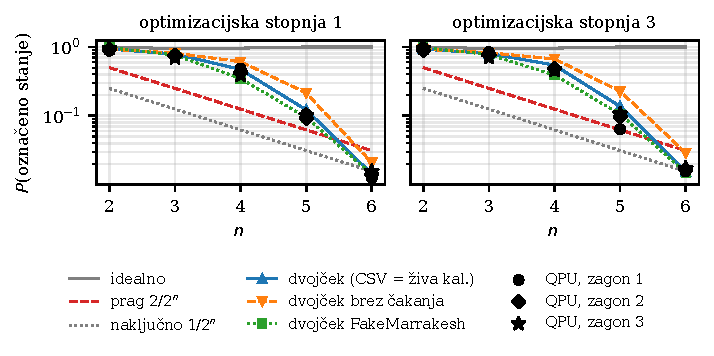
\includegraphics[width=\textwidth]{prag}
\caption{Verjetnost uspeha v odvisnosti od števila kubitov za obe optimizacijski stopnji. Dvojčki so iz zagona 3 (dvojček iz žive kalibracije je enak dvojčku iz CSV, zato ni prikazan posebej), procesor iz vseh treh zagonov. Prag $2/2^n$ (rdeča črtkana črta) presekajo vsi viri med $n = 5$ in $n = 6$.}
\label{g16:fig:prag}
\end{figure}

\begin{table}[htbp]
\caption{Verjetnost uspeha $P$ (zagon 3, stopnja 1 / 3) in razpon $P$ na procesorju čez vse tri zagone. Prag je $2/2^n$.}
\label{g16:tab:rezultati}
\centering
\begin{tabular}{rrcccc}
\toprule
$n$ & prag & QPU (zagon 3) & QPU (zagoni 1--3) & dvojček CSV & brez čakanja \\
\midrule
2 & \num{0,500} & \num{0,958} / \num{0,955} & \num{0,888}--\num{0,974} & \num{0,931} / \num{0,928} & \num{0,931} / \num{0,928} \\
3 & \num{0,250} & \num{0,697} / \num{0,703} & \num{0,697}--\num{0,843} & \num{0,790} / \num{0,807} & \num{0,812} / \num{0,823} \\
4 & \num{0,125} & \num{0,390} / \num{0,462} & \num{0,390}--\num{0,484} & \num{0,472} / \num{0,543} & \num{0,609} / \num{0,668} \\
5 & \num{0,0625} & \num{0,101} / \num{0,106} & \num{0,064}--\num{0,106} & \num{0,122} / \num{0,137} & \num{0,215} / \num{0,227} \\
6 & \num{0,031} & \num{0,016} / \num{0,017} & \num{0,013}--\num{0,017} & \num{0,014} / \num{0,015} & \num{0,021} / \num{0,029} \\
\bottomrule
\end{tabular}
\end{table}

\textbf{Število vrat.} Slika~\ref{g16:fig:vrata} prikazuje $P \cdot 2^n$ v odvisnosti od števila vrat CZ po prevajanju. Pri 37--189 vratih CZ ($n = 3$ in $4$) je rezultat na procesorju \num{5,6}- do \num{7,7}-krat boljši od naključnega ugibanja (pri $n = 2$ je največja možna vrednost 4), pri okoli 520 vratih ($n = 5$) 2- do \num{3,4}-krat, pri \num{1800}--\num{2100} vratih ($n = 6$) pa \num{0,8}- do \num{1,1}-krat. Prag torej leži med okoli 500 in \num{1800} vrati CZ. Natančneje ga s temi vezji ne moremo določiti, ker se stopnji 1 in 3 pri istem $n$ razlikujeta le za 6 do 18~\% vrat.

\begin{figure}[htbp]
\centering
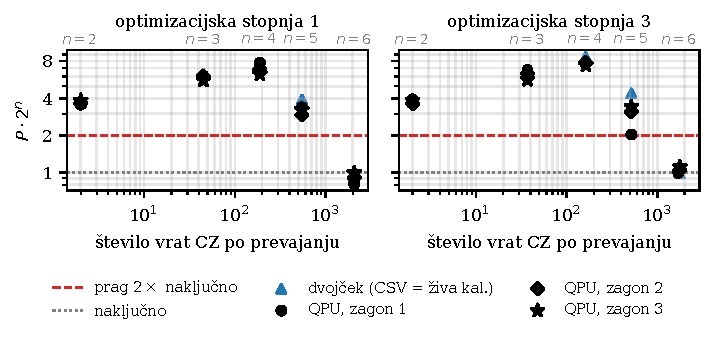
\includegraphics[width=\textwidth]{vrata}
\caption{Izboljšava nad naključnim ugibanjem $P \cdot 2^n$ v odvisnosti od števila vrat CZ po prevajanju (obe osi logaritemski). Pri $n = 6$ so vsi zagoni na ravni naključnega ugibanja.}
\label{g16:fig:vrata}
\end{figure}

\textbf{Optimizacijska stopnja.} Na istih kubitih je stopnja 3 pri $n = 4$ izboljšala rezultat s \num{0,390} na \num{0,462} (zagon 3) oziroma s \num{0,429} na \num{0,484} (zagon 2), pri $n = 3$ in $n = 5$ pa je razlika manjša od razlik med zagoni.

\textbf{Dvojčki.} Pri zagonu 3 sta bila posnetek žive kalibracije in preneseni CSV iz istega trenutka (17:26:41 UTC) in sta se ujemala v vseh \num{1072} vrednostih kubitov in vseh napakah vrat CZ, zato dvojčka iz žive kalibracije in iz CSV dasta enake rezultate. Za $n \geq 3$ vsi dvojčki z istim časom kalibracije precenijo $P$ (slika~\ref{g16:fig:cakanje}, levo). Pri $n = 4$ in $n = 5$ ga dvojček s čakanjem preceni za \num{1,18}- do \num{1,29}-krat, kontrola brez čakanja pa za \num{1,45}- do \num{2,14}-krat. Upoštevanje čakanja izboljša tudi uteženi Jaccard: pri $n = 4$ z \num{0,64}--\num{0,66} na \num{0,84}--\num{0,85} in pri $n = 5$ z \num{0,71}--\num{0,74} na \num{0,85}--\num{0,87} (slika~\ref{g16:fig:cakanje}, desno). Vsi dvojčki ostanejo pod mejo vzorčenja (\num{0,94}--\num{0,97} pri $n = 4$ in $5$), torej razlik do procesorja ne pojasni vzorčni šum. Dvojček FakeMarrakesh je bil pri zagonu 3 procesorju najbližje (\num{0,85}- do \num{0,99}-krat), verjetno zato, ker so stari podatki za izbrane kubite slabši od aktualnih in tako po naključju nadomestijo manjkajoče napake (glej razdelek~\ref{g16:sec:razprava}).

\begin{figure}[htbp]
\centering
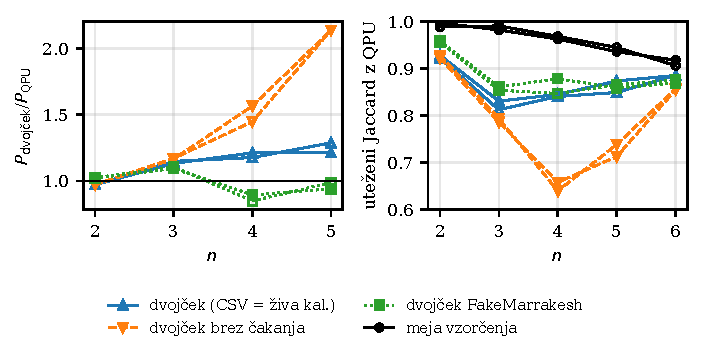
\includegraphics[width=\textwidth]{cakanje}
\caption{Levo: razmerje med verjetnostjo uspeha dvojčka in procesorja (zagon 3). Desno: uteženi Jaccard med dvojčkom in procesorjem ter meja vzorčenja. Polni znaki: stopnja 1, prazni: stopnja 3.}
\label{g16:fig:cakanje}
\end{figure}

\textbf{Klasična primerjava.} Tabela~\ref{g16:tab:klasicno} primerja povprečno število poizvedb. Idealni Groverjev algoritem je hitrejši od klasičnega iskanja pri vseh $n$, na procesorju pa le do $n = 3$; pri $n = 4$ sta enakovredna, pri $n = 5$ pa algoritem na procesorju potrebuje skoraj trikrat več poizvedb kot klasično iskanje.

\begin{table}[htbp]
\caption{Povprečno število poizvedb, da najdemo in preverimo označeni element (zagon 3, stopnja 3).}
\label{g16:tab:klasicno}
\centering
\begin{tabular}{rrrr}
\toprule
$n$ & klasično $(N+1)/2$ & idealni Grover $(k+1)/P_\mathrm{ideal}$ & Grover na QPU $(k+1)/P$ \\
\midrule
2 & \num{2,5} & \num{2,0} & \num{2,1} \\
3 & \num{4,5} & \num{3,2} & \num{4,3} \\
4 & \num{8,5} & \num{4,2} & \num{8,7} \\
5 & \num{16,5} & \num{5,0} & \num{47,0} \\
6 & \num{32,5} & \num{7,0} & \num{402} \\
\bottomrule
\end{tabular}
\end{table}


\section{Razprava}
\label{g16:sec:razprava}

\textbf{Odgovor na raziskovalno vprašanje.} Na procesorju \texttt{ibm\_marrakesh} daje Groverjev algoritem uporaben rezultat do $n = 5$ in preneha pri $n^* = 6$, kar se ujema s hipotezo ($5 \pm 1$). Prag se je ponovil v treh nalogah na različnih skupinah kubitov. Vsi digitalni dvojčki ga napovejo pravilno. Hipoteza, da dvojček verjetnost uspeha precenjuje, se je potrdila za vse dvojčke z aktualno kalibracijo, a velikost precenitve je odvisna od modela: največji del razlike pojasni dekoherenca med čakanjem kubitov. Pri $n = 5$ traja vezje (zagon 3) okoli \SI{56}{\micro\second}; trije kubiti od tega čakajo 71--73~\%, torej okoli \SI{40}{\micro\second}, kar je pri njihovih časih $T_2$ (\SIrange{128}{243}{\micro\second}) znaten del koherenčnega časa. Brez tega dela model verjetnost uspeha preceni za več kot dvakrat. Ker se $P$ med $n = 5$ in $n = 6$ zmanjša za faktor 6, napako modela za faktor 2 prag še prenese, za napoved same verjetnosti pa model brez čakanja ni primeren.

Praktično je prag še nižji od praga $2/2^n$: ob štetju poizvedb (tabela~\ref{g16:tab:klasicno}) je algoritem na procesorju hitrejši od klasičnega iskanja le do $n = 3$.

\textbf{Omejitve.} (i)~Za vsak $n$ smo uporabili eno označeno stanje; od njega je odvisno le število vrat $X$ v oraklju, kar je zanemarljivo v primerjavi s stotinami vrat CZ. (ii)~Uporabili smo en procesor. (iii)~Rezultat na procesorju se med zagoni na istih kubitih spreminja za okoli $\pm\num{0,05}$ (pri $n = 3$ in stopnji 1 \num{0,758}, \num{0,752} in \num{0,697}). (iv)~Tudi dvojček s čakanjem ostane pod mejo vzorčenja; preostale razlike verjetno izvirajo iz presluha med kubiti, koherentnih napak, uhajanja iz računske baze in spreminjanja kalibracije med izvajanjem, česar model ne vsebuje. (v)~Dobro ujemanje dvojčka FakeMarrakesh v zagonu 3 ni sistematično: v zagonu 2 (dvojčki takrat še brez čakanja) je na drugih kubitih precenil $P$ podobno kot ostali dvojčki. (vi)~Prag je odvisen od izvedbe oraklja: s pomožnimi kubiti bi bilo vrat manj in prag višji. (vii)~Klasična primerjava šteje le poizvedbe, ne pa časa prevajanja in izvajanja.

\subsection{Kaj ni delovalo}
\label{g16:sec:neuspehi}

\textbf{Prvi model iz CSV je bil \enquote{pravilen iz napačnega razloga}.} Naš prvi dvojček iz CSV je model šuma gradil ročno: vsakim vratom je dodal termično relaksacijo in depolarizacijo z napako iz CSV. Ker napaka iz CSV že vsebuje dekoherenco med vrati, je bil ta del štet dvakrat, čakanja pa model ni upošteval. V zagonu 2 je pri $n = 5$ napovedal $P = \num{0,148}$ / \num{0,160} in bil procesorju (\num{0,092} / \num{0,097}) bližje kot dvojček iz žive kalibracije brez čakanja (\num{0,212} / \num{0,226}), vendar le zato, ker sta se napaki delno izničili. Nadomestili smo ga s standardno konstrukcijo z razporejanjem.

\textbf{Stopnja 3 je brez skupne postavitve izbrala slabše kubite.} V zagonu 1 sta stopnji 1 in 3 kubite izbirali neodvisno. Stopnja 3 je pri $n = 5$ izbrala kubite 9--12 in 18, ki so imeli po kalibraciji boljša vrata CZ, in vsi dvojčki so zanjo napovedali višjo verjetnost uspeha kot za stopnjo 1 (dvojček iz žive kalibracije \num{0,304} proti \num{0,212}). Na procesorju je bilo obratno (\num{0,064} proti \num{0,105}): kubiti 9--11 so dali skoraj naključne bite. Primerjava stopenj je tako primerjala dele čipa, zato smo v zagonih 2 in 3 stopnji 3 predpisali postavitev stopnje 1.

\textbf{Napačni kalibracijski podatki.} CSV z 21.\,11.\,2026 je za kubita 0 in 1 navajal verjetnost napačnega odčitavanja stanja $\ket{0}$ \num{0,39} in \num{0,70}. Na teh kubitih sta pri $n = 2$ pristali obe stopnji v zagonu 2; dvojčka iz kalibracije sta napovedala $P = \num{0,43}$--\num{0,53}, procesor pa je dal \num{0,90}--\num{0,91}. V CSV z 22.\,11.\,2026 sta bili ti verjetnosti \num{0,002} in \num{0,113} in dvojček je v zagonu 3 na istih kubitih pri $n = 2$ napovedal \num{0,93} (procesor \num{0,96}). Dvojček je torej lahko le tako dober kot kalibracijski podatki.


\section{Zaključek}
\label{g16:sec:zakljucek}

Groverjev algoritem na procesorju IBM Heron (\texttt{ibm\_marrakesh}) daje uporaben rezultat do $n = 5$ kubitov (okoli 520 vrat CZ, $P$ okoli \num{0,1}) in preneha pri $n = 6$ (\num{1800}--\num{2100} vrat CZ, $P$ na ravni naključnega ugibanja); hitrejši od klasičnega iskanja je le do $n = 3$. Digitalni dvojčki iz kalibracijskih podatkov prag napovejo pravilno, verjetnost uspeha pa precenijo, najbolj, če ne upoštevajo dekoherence kubitov med čakanjem. Delo bi lahko nadaljevali z izvedbo oraklja s pomožnimi kubiti in z več vrednostmi $k$, s čimer bi prag določili natančneje, ter z dodajanjem presluha in koherentnih napak v model dvojčka.


\section*{Doprinosi avtorjev}

To nalogo sem izdelal sam.

\section*{Izjava o uporabi generativne umetne inteligence}

Pri delu sem uporabil Claude (Anthropic) v okolju Claude Code za pomoč pri pisanju in preverjanju kode (gradnja vezij, modeli šuma, analiza in grafi), pri iskanju napak v modelu šuma, pri preverjanju virov in pri osnutku besedila poročila. Vse rezultate, izračune in besedilo sem pregledal in preveril sam.
